\chapter{Обучение с подкреплением}\label{chap1}

Методы обучения с подкреплением являются классом методов машинного обучения. В своей основе они предполагают отсутствие учителя и знаний о среде. Таким образом им не требуется наличие источника с базой примеров правильного поведения для обучения, в связи с чем они являются самыми эффективными для задач из теории игр (шахматы, го и другое).

В рамках задачи обучения с подкреплением перед агентом стоит задача о нахождении эффективной стратегии поведения в среде, дающей максимальное суммарное вознаграждение. Основным способом обучения  в этом методе является непосредственное взаимодействие со средой, когда агент методом проб и ошибок, от попытки к попытке, улучшает свою стратегию поведения в среде. Такая идея возникла на основе наблюдения за ребенком, который обучается за счет эмпирических данных, полученных от контакта с окружающей средой. 

Одним из самых первых выдающихся результатов данного метода является программа TG-Gammon, которая учится играть в нарды. В результате обучения программа смогла играть с действующими на тот момент чемпионами в нарды \cite{nards}. Кроме того анализ ее стратегий способствовал изменению общепринятых способов разыгрывания партий. 
 
%%%%%%%%%%%%%%%%%%%%%%%%%%%%%%%%%%%%%%%%%%%%%%%%%%%%%%%%%%%%%%%%%%%%%%%%%%%%%%%%
\section{Основные понятия обучения с подкреплением}\label{1sec:optimal-control}
%%%%%%%%%%%%%%%%%%%%%%%%%%%%%%%%%%%%%%%%%%%%%%%%%%%%%%%%%%%%%%%%%%%%%%%%%%%%%%%%

Целью методов обучения с подкреплением является обучение агента,
взаимодействующего с окружающей средой. В основе данного обучения лежит гипотеза о вознаграждении: любая цель может быть описана с помощью задачи о максимизации ожидаемого совокупного вознаграждения.


\definition{Вознаграждение, или подкрепляющий сигнал (reward, $r$),  – это число, отражающее, насколько удачно поведение агента на текущем шаге.} 


Таким образом задача агента – максимизировать общее вознаграждение. Для этого агенту нужно научиться выбирать последовательность действий,  которые принесут максимальную награду. Важно, что награда может быть отложенной, если действие удачное и вызывает долгосрочные последствия. Поэтому иногда нет смысла обращать внимание на мгновенное вознаграждение и следить за долгосрочной наградой. Например, для задачи инвестирования в ценные бумаги необходимо подождать как минимум неделю, чтобы понять привело ли действие к прибыли. 

В основе обучения с подкреплением лежит модель агент-среда (рисунок 2.1). Исходя из нее агент может понимать свое текущее состояние в среде (current state, $s$), наблюдать окружающее пространство (observation, $o$), на основе наблюдений предпринимать действия (actions, $a$), переходить в новое состояние и получать вознаграждение (reward, $r$). Схематически это можно увидеть на рисунке ~\ref{fig:ag-en}.

\begin{figure}[!h]
	\centering
	\includegraphics[scale=0.42]{agent_env.png}	
	\caption {Агент и среда}
	\label{fig:ag-en}
\end{figure}

Агент взаимодействует со средой в дискретные моменты времени $t=0, 1, \dots$.

В каждый момент времени $t$ агент получает информацию о состоянии среды $$s_t \in S, $$ где $S$ – множество состояний среды. Состояние может включать в себя
низкоуровневые параметры (силу тока) и
высокоуровневые (текущее время). Также внутренние параметры агента могут входить в состояние среды, то есть граница
между средой и агентом не всегда совпадает с их физической границей.


Далее агент выбирает действие на основе состояния: $$a_t \in A(s),$$ 
где $A(s)$ – множество возможных действий, доступных в состояния $s$.

После исполнения действия агент получает новое состояние $s_{t+1}$, и награду $r_{t+1}$. 

Такую модель действий агента обычно называют моделью с обратной связью \cite{rl1}.


Выбор агента о том, какое действие предпринять, основывается на истории. \definition{Историей $h_t$ называют последовательность из действий, наблюдений и вознаграждений агента до момента времени $t$.}
\begin{equation}
    h_t = \{a_1, s_1, r_1, \dots, a_t, s_t, r_t\}.
    \label{eq:hist}
\end{equation}

В ответ на действие среда возвращает наблюдение и награду, которые записываются в историю. Таким образом состояние среды является функцией от истории (\ref{eq:hist}):
$$s_{t+1} = f(h_t)$$

В рамках нашей задачи агент получает полное состояние окружающей среды, причем оно  является марковским.

\definition{Состояние называется марковским тогда и только тогда, когда выполнено свойство марковости: }
$$P[s_{t+1} | s_t] = P[s_{t+1} | s_1, \dots, s_t],$$
т.е. будущее состояние $s_{t+1}$ зависит только от текущего состояния $s_t$ и не зависит от прошлых. Таким образом, зная текущее состояние, все дальнейшие состояния могут быть получены без знания истории. 
 
 Свойства марковских процессов (Markov decision process – MDP), повзоляют формально описывать среду и её модели для различных видов задач обучения с подкреплением.

MDP описывается пятью параметрами $(S, A, {P^a_s},\gamma, R)$: 
\begin{itemize}
    \item S -- множество возможных состояний системы,
    \item A --  множество действий агента,
    \item $P_s^a$ -- матрица вероятностей перехода между состояниями. Т. е. состоящую из вероятностей $P^a_{ss'}$ перехода из состояния $s\in S$  в состояние $s' \in S$ , предприняв действие $a \in A$.  
    \item $\gamma$ -- дисконтирующий множитель. С помощью него отражается задержка в награде. $\gamma \in [0, 1],$
    \item $R$ - функция наград. $R : S \times A \to \mathbb{R}$ :
    $$R_s^a = \mathbb{E} [ r_{t+1} | r_t = s, r_t = a].$$
\end{itemize}

Пример диаграммы переходов для марковского процесса принятия решений можно увидеть на рисунке ~\ref{fig:mdp-pic}. \newpage

\begin{figure}[h]
	\centering
	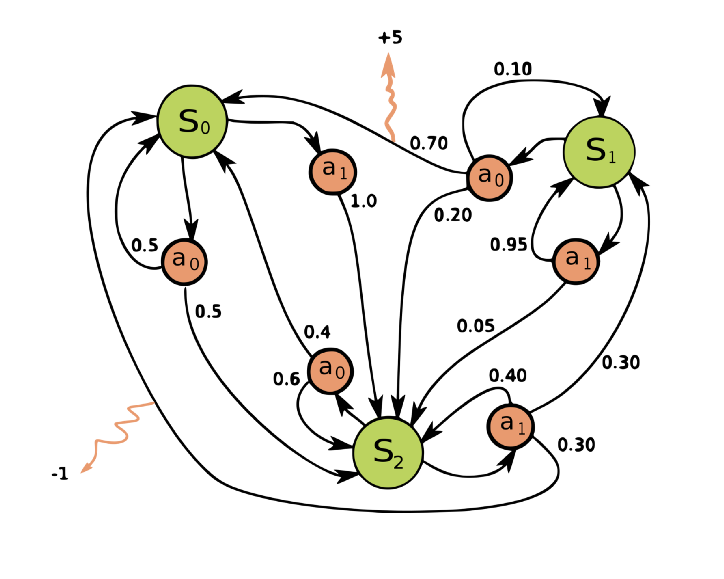
\includegraphics[scale=0.6]{mdp_pic.png}
	\caption {Марковский процесс принятия решений}	
	\label{fig:mdp-pic}
\end{figure}


Среда для маятника является непрерывной и сводится к MDP при помощи техники дискретизации \cite{rl2}.

\definition{Доходом $g_t$ называется случайная величина, равная дисконтированной сумме вознаграждений агента после момента времени $t$}.
\begin{equation}
    g_t = r_{t+1} + \gamma r_{t+2} + \gamma^2 r_{t+3} + \dots = \sum\limits_{k=1}^{\infty} \gamma^k r_{t+k}.
    \label{eq:doh}
\end{equation}


\definition{Гипотеза о награде Сьюттона: вместо максимизации суммарной награды можно ставить агенту целью максимизациой суммы наград, полученных на последующих шагах при выборе текущего действия.}

Таким образом задачу агента можно переопределить как максимизацию ожидания дохода (\ref{eq:doh}).



 
%%%%%%%%%%%%%%%%%%%%%%%%%%%%%%%%%%%%%%%%%%%%%%%%%%%%%%%%%%%%%%%%%%%%%%%%%%%%%%%%
\section{Структура агента}\label{1sec:optimal-control}
%%%%%%%%%%%%%%%%%%%%%%%%%%%%%%%%%%%%%%%%%%%%%%%%%%%%%%%%%%%%%%%%%%%%%%%%%%%%%%%%

В задаче оптимального управления ключевыми являются три следующие компоненты: 
\begin{enumerate}
    \item \textbf{Policy}  -- стратегия поведения.
    
    Стратегия $\pi$ -- это стратегия поведения агента по отношению к среде. 
    
    \textbf{Стратегия (Policy function) } – функция, которая ставит в соответствие состоянию агента предпринимаемое им действие. 
    Детерминированная стратегия имеет вид: 
    $$a = \pi(s), s \in S,$$
    Стохастическая стратегия:
    \begin{equation}
    \pi(a|s) = P[a_t = a| s_t = s].
    \label{eq:pi}
    \end{equation}

	\item \textbf{Value function} -- функция ценности действия.
    
    \textbf{Функция ценности (Value function)} –  функция, предсказывающая возможное вознаграждение, которое получит агент, находящийся в момент $t$ в состоянии $s_t$.
    
    \begin{equation}
    	\nu(s) = \mathbb{E} [ r_t + \gamma r_{t+1} + \gamma^2 r_{t+2} + \dots | s_t = s].
    	\label{eq:nu}
    \end{equation}
    
    (\ref{eq:nu}) также можно определить через доход (\ref{eq:doh}):
    \begin{equation}
    	\nu(s) = \mathbb{E}[g_t | s_t = s].
    	  \label{eq:nu2}
    \end{equation}
    
    \item\textbf{Model} --  модель среды.
    
    \textbf{Модель среды} –  модель, которая предсказывает что будет со средой в следующий момент времени.
    
    В основе модели лежат модель переходов и модель вознаграждений, которые показывают вероятность следующего состояния в зависимости от текущего и ожидаемую награду соответственно:
    
    \begin{equation}
    	\Phi_{ss'}^a = P[s_{t+1} = s'| s_t = s, a_t = a],
    	\label{eq:phi}
    \end{equation}
	\begin{equation}
	\Psi_{s}^a = E[r| s_t = s, a_t = a].
	\label{eq:psi}
	\end{equation}
	Сама же модель среды описывается как функция: 
	\begin{equation}
		s_{t+1} = m(s_t, a_t).
		\label{eq:model}.
	\end{equation}
    
\end{enumerate}



\definition{Функция стоимости действия (action-value function) Марковского процесса принятия решений – есть ожидаемый доход, начиная с состояния $s$, при принятии действия $a$ и в дальнейшем следуя стратегии $\pi$.}

\begin{equation}
    q_{\pi} (s, a)= \mathbb{E_{\pi}} [g_t | s_t = s, a_t = a].
    \label{eq:qu}
\end{equation}

На основе введенных определений (\ref{eq:pi}) и (\ref{eq:nu2})  помощью уравнения Беллмана выводится следующее представление:


\begin{equation}
	\nu_{\pi}(s, a) = \mathbb{E_\pi} [ r_{t+1} + \gamma \nu_\pi(s_{t+1}) | s_t=s],
	\label{eq:nu3}
\end{equation}

Из (\ref{eq:qu}) и (\ref{eq:nu3}) получается следующий удобный вид функции $q)$:

\begin{equation}
    q_{\pi}(s, a) = \mathbb{E_\pi} [ r_{t+1} + \gamma q_\pi(s_{t+1}, a_{t+1}) | s_t=s, a_t=a].
    \label{eq:q2}
\end{equation}


 
%%%%%%%%%%%%%%%%%%%%%%%%%%%%%%%%%%%%%%%%%%%%%%%%%%%%%%%%%%%%%%%%%%%%%%%%%%%%%%%%
\section{Q-обучение}\label{1sec:optimal-control}
%%%%%%%%%%%%%%%%%%%%%%%%%%%%%%%%%%%%%%%%%%%%%%%%%%%%%%%%%%%%%%%%%%%%%%%%%%%%%%%%

\definition{Q-learning (q-обучение) — это один из алгоритмов реализации метода машинного обучения с подкреплением (reinforcement learning, RL). Часто используется в задачах, в которых отсутствует модель среды.}

Задача обучения с подкреплением формулируется как нахождение стратегии $\pi^*(s)$, которая максимизирует математическое ожидание дохода (\ref{eq:nu2}): $\mathbb{E}[g_t] \to \max$ . Тогда оптимальную стратегию в текущем состоянии $s$ можно записать: 
\begin{equation}
    \pi^*(s) = \arg \max_a{q(s, a)}.
    \label{eq:pi2}
\end{equation}

На основе (\ref{eq:qu}) и (\ref{eq:pi2}) введем следующую функцию:

\begin{equation}
	q^*_{\pi}(s, a) = \mathbb{E}_{\pi^*} [g_t|s_t=s, a_t=a]
	\label{eq:qu**}
\end{equation}
 
Таким образом вместо поиска $\pi^*(s)$ наша задача сводится к поиску $q^*(s, a)$


Используя формулу (\ref{eq:q2}) и на основе (\ref{eq:qu**}) метод аппроксимирует значения оптимальной функции выигрыша $q^*$ следующим образом:

\begin{equation}
	\begin{split}
    q^*_{\pi}(s, a) = \mathbb{E_\pi} [ r_{t+1} + \gamma q_\pi(s_{t+1}, a_{t+1}) | s_t=s, a_t=a] = \\
     \frac{1}{N} \left( \sum\limits_{i} r_i + \gamma \max_{a'} q(s^{next}_i, a') \right) = \\ \dots.
    \end{split}
	\label{eq:qu*}
\end{equation}

Алгоритм состоит из следующих шагов:
\begin{itemize}
    \item Произвольно инициализируются $a, s, r, s'$, функция  $q(s, a) \forall s \in S, a \in A$.
    \item Рассматриваются возможные действия $a$ и находится новое действие $a' = \arg \max\limits_{a \in A}q(s', a) $.
    \item Берется среднее взвешенное от уже имеющейся функции стоимости и подсчитанной на текущем шаге на основе (\ref{eq:qu*}):  
    
    \begin{equation}
    	q(s, a) = \gamma [R(s, a) +\gamma q(s', a')] + (1-\gamma)q(s, a).
    	\label{eq:qu3}
    \end{equation}
\end{itemize}

Схему работы алгоритма  q-обучения можно увидеть на рисунке ~\ref{fig:q-learn}. \newpage

\begin{figure}[h]
	\centering
	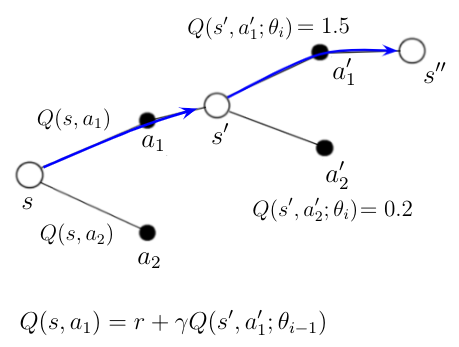
\includegraphics[scale=1]{q_learn.png}
	\caption {Пересчет $q(s, a)$}
	\label{fig:q-learn}
\end{figure}

В качестве метода аппроксимации функции $q(s', a')$ из (\ref{eq:qu3}) часто используется нейронная сеть. Для  оптимизации в качестве функции ошибки выбирается следующая:

$$L = \frac{1}{N} \sum\limits_{i=1}^N \left( q(s, a) - [r(s, a) + \gamma \max_{a'} q(s', a')]^2  \right),$$
где $s, a, R, s'$ -- текущее состояние, действие, награда и следующее состояние соответственно. 

Сама нейронная сеть для $q(s', a')$ представлена на рисунке ~\ref{fig:q-l}. 

\begin{figure}[h]
	\centering
	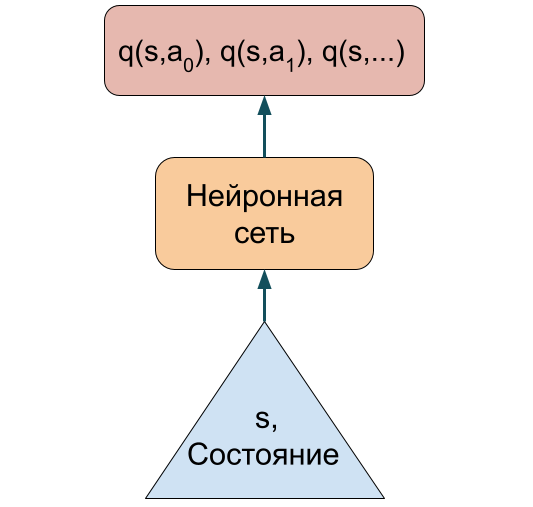
\includegraphics[scale=0.6]{q_l.png}
	\caption {Модель обучения нейронной сети}
	\label{fig:q-l}
\end{figure}
\newpage


%%%%%%%%%%%%%%%%%%%%%%%%%%%%%%%%%%%%%%%%%%%%%%%%%%%%%%%%%%%%%%%%%%%%%%%%%%%%%%%%
\section{Eпсилон-жадный алгоритм}\label{1sec:optimal-control}
%%%%%%%%%%%%%%%%%%%%%%%%%%%%%%%%%%%%%%%%%%%%%%%%%%%%%%%%%%%%%%%%%%%%%%%%%%%%%%%%

В рамках подхода q-обучения всегда выбирается действие в зависимости от получаемой награды. Таким образом политика агента заключается в выборе такого действия, которое в тот же момент времени принесет максимальную возможную награду в данном состоянии (\ref{eq:pi2}). Однако иногда суммарный доход будет больше, если в текущем состоянии взять не максимальную награду, но попасть в состояние, из которого в дальнейшем можно получить награду намного больше.

В рамках эпсилон-жадного алгоритма действий агент не только использует накопленные знания, но и немного исследует среду. Эпсилон-жадный алгоритм большую часть времени выбирает действие с максимальной наградой. Цель его состоит в том, чтобы найти баланс между выбором нового и локально оптимального. 

Данный подход заключается в том, чтобы с небольшой вероятностью $\epsilon$ производить исследование среды  -- выбирать случайное действие. А с вероятностью $1-\epsilon$ выбирать действие с максимальной наградой. Схематически это представлено на рисунке ~\ref{fig:eps}. \newpage


\begin{figure}[h]
	\centering
	\includegraphics[scale=0.55]{e-gr.png}
	\caption {Эпсион-жадный алгоритм.}
	\label{fig:eps}
\end{figure}


%%%%%%%%%%%%%%%%%%%%%%%%%%%%%%%%%%%%%%%%%%%%%%%%%%%%%%%%%%%%%%%%%%%%%%%%%%%%%%%%
\section{Выводы}\label{1sec:optimal-control}
%%%%%%%%%%%%%%%%%%%%%%%%%%%%%%%%%%%%%%%%%%%%%%%%%%%%%%%%%%%%%%%%%%%%%%%%%%%%%%%%


В рамках данной главы была дана общая характеристика обучения с подкреплением. Была описана модель агент-среда, марковский процесс принятия решений и представлен алгоритм q-обучение для решения поставленной задачи. Также было описано его улучшение в виде эпсилон-жадного алгоритма.
